\documentclass[12pt]{book}
%\usepackage[width=4.375in, height=7.0in, top=1.0in, papersize={5.5in,8.5in}]{geometry}
\usepackage[a4paper]{geometry}
\usepackage[pdftex]{graphicx}
\usepackage{amsmath}
\usepackage{amssymb}
\usepackage{tipa}
\usepackage{textcomp}
\usepackage{fancyhdr}
\usepackage{latexsym}
\usepackage{paralist}
\usepackage{comment}
\usepackage{fancyvrb}
\usepackage{multirow}
\usepackage{url}
\usepackage[group-separator={,}]{siunitx}
\usepackage{pgfplots}

\usetikzlibrary{arrows.meta} \pagestyle{plain}
\pgfplotsset{compat=1.12}

\pagestyle{fancy}
\renewcommand{\chaptermark}[1]{\markboth{#1}{}}
\renewcommand{\sectionmark}[1]{\markright{\thesection\ #1}}
\fancyhf{}
\fancyhead[LE,RO]{\bfseries\thepage}
\fancyhead[LO]{\bfseries\rightmark}
\fancyhead[RE]{\bfseries\leftmark}
\renewcommand{\headrulewidth}{0.5pt}
\renewcommand{\footrulewidth}{0pt}
\addtolength{\headheight}{0.5pt}
\setlength{\footskip}{0in}
\renewcommand{\footruleskip}{0pt}
\fancypagestyle{plain}{%
\fancyhead{}
\renewcommand{\headrulewidth}{0pt}
}
%
%\parindent 0in
\parskip 0.05in
%

\includecomment{solution}
%\excludecomment{solution} % comment this out to create the solutions
\newcommand{\bs}{\textbf{Solution.}~}
\newcommand{\es}{\hfill  $\square$}

\setcounter{secnumdepth}{2}

\begin{document}
\frontmatter
%
\chapter*{\Huge \center An Introduction to Prescriptive and Predictive Modeling }
\thispagestyle{empty}
%{\hspace{0.25in} \includegraphics{./ru_sun.jpg} }
%\section*{\large \center Darin England}
\newpage
\subsection*{\center \normalsize Copyright \copyright 2020 by Darin England}
\subsection*{\center \normalsize All rights reserved.}
\subsection*{\center \normalsize ISBN \dots}
\subsection*{\center \normalsize \dots Publications}
%
%\chapter*{\center \normalsize To my Son}
%
\tableofcontents
%
\mainmatter
%
\chapter{Prescriptive Modeling}
\section{Linear Programming}

% this section needs to be re-written
\emph{A Resource Allocation Problem.} This example is taken 
from~\cite{chvatal:1983}.  A forester has 100
acres of hardwood timber. She also has \$4000 cash on-hand to use for
the forestry business. There are two possible courses of action to
take with the 100 acres of available hardwood:
\begin{enumerate}
\item Harvest the hardwood and let the area naturally regenerate. This
  would cost \$10 per acre now and return \$50 per acre later,
  yielding a profit of \$40 per acre.
\item Harvest the hardwood and plant the area with pine. This would
  cost \$50 per acre now and return \$120 per acre later, yielding a
  profit of \$70 per acre. \label{d2}
\end{enumerate}
Option \ref{d2} is clearly more profitable; however, the forester must
respect her budget of \$4000. The mathematical programming problem is
to maximize total profit subject to the resource constraints, which
are the acres of available hardwood and the budget.

The complete problem formulation in AMPL is shown in
figure~\ref{forest}.  Two decision variables, \texttt{x1} and
\texttt{x2}, represent the number of acres that the forester should
allocate to each of the two possible courses of action.  It would make
no sense to allow these decision variables to take on negative
values. The non-negativity requirements are more cleanly specified
directly in the variable declarations as opposed to creating separate
constraints. A graphical depiction of the feasible solution space is
shown in figure~\ref{feasibleregion}.

\begin{SaveVerbatim}{vrbforest}
var x1 >= 0;  # acres to fell and let regenerate
var x2 >= 0;  # acres to fell and plant with pine

maximize profit: 40*x1 + 70*x2;

s.t. acres: x1 + x2 <= 100;
s.t. budget: 10*x1 + 50*x2 <= 4000;
\end{SaveVerbatim}

\begin{figure}
\fbox{
\begin{minipage}{\textwidth}
\BUseVerbatim{vrbforest}
\caption{Forestry problem (\texttt{forester.mod})}
\label{forest}
\end{minipage}
}
\end{figure}

\begin{figure}
\begin{center}
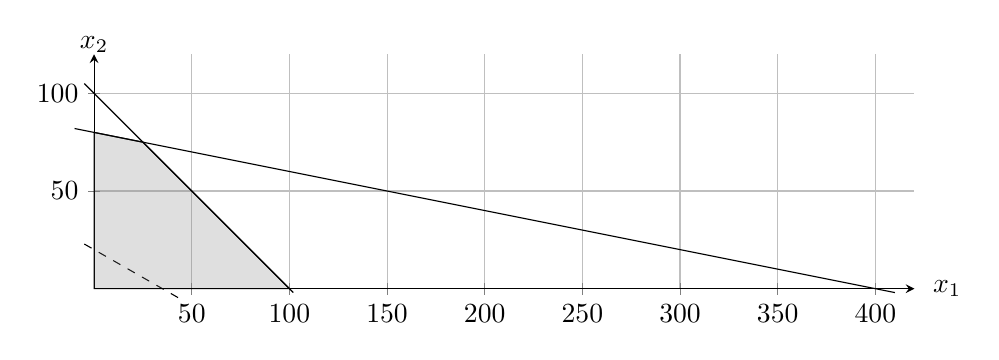
\begin{tikzpicture}
  \begin{axis}[ width=12cm,
    unit vector ratio*=1 1 1,
    enlargelimits=false,
    grid=both,
    axis x line=middle,
    axis y line=middle,
    title=,
    clip=false,
    ymin=0, ymax=120,
    xmin=0, xmax=420 ]

    \addplot[domain=-10:410] {80 - .2*x};
    \addplot[domain=-5:102] {100 - x};
    \addplot[domain=-5:45,dashed] {20 - .57143*x};
    \addplot[fill=gray, fill opacity=.25]
    coordinates { (0,0) (100,0) (25,75) (0,80) }\closedcycle;

  % to get axis labels at the end of the axis
  \node at (axis description cs:1.04,0) {$x_1$}; \node at
  (axis description cs:0,1.04) {$x_2$};
\end{axis}
\end{tikzpicture}
\end{center}
\caption{Feasible Region for the Forestry Problem}
\label{feasibleregion}
\end{figure}

The constraints labeled \texttt{acres} and \texttt{budget} represent
the limitations on available resources.  It's unnecessary to
explicitly name constraints in AMPL; however, providing short,
descriptive names aids interpretation of the model. Moreover, in a
resource allocation problem such as this, the constraint names refer
to the values of the associated dual variables, which have an economic
interpretation as the marginal value of an additional unit of the
resource.

This problem is small enough that we can include all data parameters
directly in the model specification. Although we will not cover it in
this quick start guide, it is good practice to separate the data from
the model, and AMPL encourages this separation by providing
\texttt{param} declarations and the ability to have a separate
\texttt{data} section. Indeed, it's hard to understand the benefit of
an algebraic modeling language unless you are working on a large
problem.  It's worth noting that AMPL doesn't actually solve the
mathematical programming problem, but rather passes a description of
the problem to a solver, which returns information about the solution
(if any solution was found) to AMPL. An AMPL session for the forestry
problem follows:

\begin{Verbatim}[samepage=true]
ampl: model forester.mod;
ampl: solve;
MINOS 5.5: optimal solution found.
2 iterations, objective 6250
ampl: display x1,x2;
x1 = 25
x2 = 75
\end{Verbatim}

The optimal solution indicates that the forester should let 25 acres
of the hardwood regenerate naturally and plant 75 acres with pine, for
a total profit of \$6250. Notice that the entire budget of \$4000 is
exhausted because $10 \times 25 + 50 \times 75 = 4000$. When a
resource capacity constraint such as \texttt{acres} or \texttt{budget}
holds with equality in the optimal solution (as in this example), then
the constraint is \emph{binding}; all of the resource associated with
the constraint is being consumed. If more/less of the resource were
available, then profit would be increased/decreased. The value of the
associated dual variable indicates the amount by which profit would be
affected for small changes in the supply of the resource. This is
called the marginal value of a resource, or the shadow price.

\begin{Verbatim}[samepage=true]
ampl: display acres, budget;
acres = 32.5
budget = 0.75
\end{Verbatim}

In AMPL the name of a constraint is used to refer to the associated
dual variable. Displaying the shadow prices for the forester problem
indicates that an additional acre of hardwood timber would increase
profit by \$32.50, given the same budget of \$4000.  Modifying the
right-hand side of \texttt{acres} to 101 and re-solving shows that
this is indeed the case.

\begin{Verbatim}[samepage=true]
ampl: reset;
ampl: model forester.mod;
ampl: expand acres;
subject to acres:
	x1 + x2 <= 101;

ampl: solve;
MINOS 5.5: optimal solution found.
2 iterations, objective 6282.5
ampl: display x1,x2;
x1 = 26.25
x2 = 74.75
\end{Verbatim}

The \texttt{expand} command displays the full form of a set of
constraints.  (This will be useful for indexed expressions.) Notice
that the values of the decision variables have necessarily changed and
that the solution is no longer integer-valued.  This is typical of
resource allocation problems. We are in fact assuming that the
forester is able to execute the decisions on partial acres.  For the
\texttt{budget} constraint, an additional one dollar increase/decrease
in the right-hand side would increase/decrease profit by \$0.75, given
the same 100 acres of hardwood. It stands to reason, then, that the
forester could take out a loan and apply the funds to her
operation. As long as the interest rate is less than .75, profit will
increase.

Shadow prices are valid for \emph{limited} increases/decreases in the
right-hand sides of the constraints. The ranges over which the these
values are valid is a topic of sensitivity analysis. Here, we will
show how to extract this information from AMPL. First we need to tell
AMPL to use a solver that is able to return sensitivity information
along with the optimal solution. We will instruct AMPL to use the solver
\texttt{gurobi}. Then we set a solver-specific option to make the
sensitivity range information available.

\begin{Verbatim}[samepage=true]
ampl: reset;
ampl: model forester.mod;
ampl: option solver gurobi;
ampl: option gurobi_options 'solnsens 1'; 
ampl: solve;
Gurobi 8.1.0: solnsens 1
Gurobi 8.1.0: optimal solution; objective 6250

suffix sensublo OUT;
suffix sensubhi OUT;
suffix sensobjlo OUT;
suffix sensobjhi OUT;
suffix senslblo OUT;
suffix senslbhi OUT;
suffix sensrhslo OUT;
suffix sensrhshi OUT;
\end{Verbatim}

We are now able to display the ranges over which the current shadow
prices of \$32.5 per acre and \$0.75 per dollar of budget are
valid. To do this we simply add a suffix to the name of the
constraint, separated by a ``\texttt{.}''. The suffix
\texttt{.sensrhslo} displays the lower limit of a constraint's
right-hand side, while \texttt{.sensrhshi} displays the upper limit.
In the AMPL session follows, the
upper limit of 5000 on the right-hand side of \texttt{budget}
indicates the forester should only consider loans of \$1000 or less to
be valued at an incremental marginal value of 0.75.

\begin{Verbatim}[samepage=true]
ampl: display acres.sensrhslo, acres.sensrhshi;
acres.sensrhslo = 80
acres.sensrhshi = 400

ampl: display budget.sensrhslo, budget.sensrhshi;
budget.sensrhslo = 1000
budget.sensrhshi = 5000
\end{Verbatim}

Sensitivity ranges may also be obtained for the decision variables. In
this case the lower and upper limits represent the valid ranges on the
objective function coefficients over which the current solution
remains optimal.  The suffixes \texttt{.sensobjlo} and
\texttt{.sensobjhi} are used to refer to these lower and upper limits.
Displaying this information for the forestry problem reveals that the
current solution value of \texttt{x1 = 25} remains optimal as long as
its coefficient in the objective function is in the range 14 to 70,
holding all other parameters at their current values.

\begin{Verbatim}[samepage=true]
ampl: display x1.sensobjlo, x1.sensobjhi;
x1.sensobjlo = 14
x1.sensobjhi = 70

ampl: display x2.sensobjlo, x2.sensobjhi;
x2.sensobjlo = 40
x2.sensobjhi = 200
\end{Verbatim}

The other suffixes, \texttt{.senslblo}, \texttt{.senslbhi},
\texttt{.sensublo}, and \texttt{.sensubhi}, refer to ranges on the
values (not the coefficients) of the decision variables over which the
current basis remains optimal. We will not use these suffixes.

\section{Integer Programming}

\section{Dynamic Programming}

\section{Inventory Models}

\section{Exercises}
\begin{enumerate}

% this exercise needs to be re-written
\item In the Ma-and-Pa grocery store, shelf space is limited
  and must be used effectively to increase profit. Two cereal items,
  Grano and Wheatie, compete for a total shelf space of 60 ft$^2$. A
  box of Grano occupies .2 ft$^2$ and a box of Wheatie requires .4
  ft$^2$. The maximum daily demands for Grano and Wheatie are 200 and 120
  boxes, respectively. A box of Grano nets \$1.00 in profit, while a
  box of Wheatie nets \$1.35. Ma and Pa think that because the unit
  profit of Wheatie is 35\% higher than that of Grano, Wheatie should
  be allocated 35\% more space than Grano, which amounts to allocating
  about 57\% to Wheatie and 43\% to Grano. What do you think?
  (You can solve this problem however you like, but you must provide
  the allocation of shelf space that maximizes profit.)

\begin{solution}
\bs My AMPL model and output follow. The solution indicates that more
space should be allocated to Grano than Wheatie. This is because
the profit per square foot is larger. The solution indicates that
Ma and Pa should stock 200 boxes of Grano and 50 boxes of Wheatie.

\begin{Verbatim}[samepage=true]
var x1 >=0, <= 200;   # boxes of grano
var x2 >= 0, <= 120;  # boxes of wheatie

maximize profit: x1 + 1.35*x2;
s.t. space: .2*x1 + .4*x2 <= 60;

ampl: model '/home/darin/Dropbox/isye/ie1101/hw/ma-and-pa-store.mod';
ampl: solve;
MINOS 5.51: optimal solution found.
2 iterations, objective 267.5
ampl: display x1, x2;
x1 = 200
x2 = 50
\end{Verbatim}
\end{solution}
\end{enumerate}

%  
\chapter{Probabilistic Modeling}

\section{Stochastic Processes}

\section{Queueing Models}

\section{Exercises}

\chapter{Decision Problems}

\section{Games Against Nature}

\section{Games Against an Opponent}

\section{Exercises}
\begin{enumerate}

% This exercise is OK
\item Rules for decision--making under ignorance (that is to
  say, decision--making without probabilities). You have the opportunity to go on a
  blind date, but you are hesitant.  You are lonely and would like to
  find the love of your life; however, you dislike awkward
  situations. Furthermore, you find it difficult to estimate the
  probability that this particular blind date will turn out to be the
  love of your life, but you know this probability is
  non-negligible. To be a little more precise, you have the following
  values: finding the love of your life is worth 1000, being in an
  awkward date situation (i.e. being on a date and knowing that you
  will not see the person again) is worth -10, and staying home
  watching Netflix is worth zero.

\begin{enumerate}
\item Formulate a decision problem for deciding whether to go on the
blind date or to stay home.
\item Use the maximin rule to solve the problem.
\item Use the minimax regret rule to solve the problem.
\end{enumerate}

\begin{solution}
\bs The decision problem can be represented with the following table.
\\[.2in]
\begin{tabular}{ccc}
\multicolumn{3}{c}{decision matrix} \\
 & find love & lots of awkward moments \\ \hline
go on date & 1000 & -10 \\
decline date & 0 & 0 
\end{tabular}
\\[.2in] 
The maximin rule tells you to decline the date because it has
the best of all the worst possible outcomes. To use minimax regret, we
form the regret matrix.  \\[.2in]
\begin{tabular}{ccc}
\multicolumn{3}{c}{regret matrix} \\
 & find love & lots of awkward moments \\ \hline
go on date & 0 & -10 \\
decline date & -1000 & 0
\end{tabular}
\\[.2in] Minimax regret tells you to go on the date because the
possibility of not finding love has the most regret.
\end{solution}


% this problem needs to be re-written. It is IMS chapter 13 problem 21.
\item A real estate investor has the opportunity to purchase land currently
zoned residential. If the county board approves a request to rezone the property
as commercial within the next year, the investor will be able to lease the
land to a large discount firm that wants to open a new store on the property.
However, if the zoning change is not approved, the investor will have to sell
the property at a loss. Profits (in thousands of dollars) are shown in the 
following payoff table.

\begin{tabular}{rcc}
& \multicolumn{2}{c}{State of Nature} \\
& rezoning approved & rezoning not approved \\
Decision Alternative & $s_1$ & $s_2$ \\
purchase & 600 & -200\\
do not purchase & 0 & 0
\end{tabular}

\begin{enumerate}
    \item If the probability that rezoning will be approved is 0.5, what
    decision is recommended? What is the expected payoff?
    \item The investor can purchase an option to buy the land. Under the option,
    the investor maintains the right to purchase the land anytime during the next
    three months while learning more about possible resistance from area residents.
    Probabilities are as follows:
    
    \begin{tabular}{rrr}
    \multicolumn{3}{c}{Let $H$ = high resistance to zoning}\\
    \multicolumn{3}{c}{Let $L$ = low resistance to zoning}\\
    $P(H)=0.55$ & $P(s_1 \mid H)=0.18$ & $P(s_2 \mid H)=0.82$ \\
    $P(L)=0.45$ & $P(s_1 \mid L)=0.89$ & $P(s_2 \mid L)=0.11$ 
    \end{tabular}
    
    What is the optimal decision strategy if the investor uses the option
    period to learn more about the resistance from area residents before making
    the purchase decision?
    \item If the option will cost the investor an additional \$\num{10000}, 
    should the investor purchase the option? Why or why not? What is the maximum
    that the investor should be willing to pay for the option?
\end{enumerate}
\begin{solution}
\bs For part a), the best decision (according to expected monetary value)
is to purchase the land. The expected profit is \$200.

For part b), If there is high resistance to rezoning (H) then
purchasing the land would yield an expected profit of -\$56 (in \$1000s).
Not purchasing the land would yield zero. If there is low
resistance to rezoning (L) then purchasing the land would yield
an expected profit of \$512 (in \$1000s). Not purchasing the
land would yield zero. So the optimal decision strategy is to
not purchase the land if H and to purchase the land if L.

For part c), the expected profit from purchasing the option
(but before actually purchasing the option) is
\[ 0 \times P(H) + 512 \times P(L) = \$230.4 \]
The maximum amount that the investor should be willing to pay is
\[ \$230.4 - \$200 = \$30.4 ~\text{(in \$1000s)} \]
\end{solution}


\end{enumerate}

%
\chapter{Data Analysis and Statistics}

\section{Summarizing Data}

\section{Visualizing Data}

\section{Exercises}

%
\chapter{Predictive Modeling}

\section{Linear Regression}

\section{Time Series}

\section{Exercises}

%
\backmatter
%
\nocite{Anderson:2015pnas} % example

\bibliographystyle{plain} % We choose the "plain" reference style
\bibliography{bibdata}    % Entries are in the "bibdata.bib" file
\end{document}
